
% VLDB template version of 2020-08-03 enhances the ACM template, version 1.7.0:
% https://www.acm.org/publications/proceedings-template
% The ACM Latex guide provides further information about the ACM template

\documentclass[sigconf, nonacm]{acmart}

%% The following content must be adapted for the final version
% paper-specific
\newcommand\vldbdoi{XX.XX/XXX.XX}
\newcommand\vldbpages{XXX-XXX}
% issue-specific
\newcommand\vldbvolume{14}
\newcommand\vldbissue{1}
\newcommand\vldbyear{2020}
% should be fine as it is
\newcommand\vldbauthors{\authors}
\newcommand\vldbtitle{\shorttitle} 
% leave empty if no availability url should be set
\newcommand\vldbavailabilityurl{URL_TO_YOUR_ARTIFACTS}
% whether page numbers should be shown or not, use 'plain' for review versions, 'empty' for camera ready
\newcommand\vldbpagestyle{plain} 

\begin{document}
\title{RepEng Project: JSONSchemaDiscovery}

%%
%% The "author" command and its associated commands are used to define the authors and their affiliations.
\author{Andreas W. Weber}
\affiliation{%
  \institution{University of Passau}
  \streetaddress{Innstr. 41}
  \city{Passau}
  \state{Germany}
  \postcode{94469}
}
\email{weber236@ads.uni-passau.de}

\maketitle

%%% VLDB block start %%%
\pagestyle{\vldbpagestyle}

%%% do not modify the following VLDB block %%
%%% VLDB block start %%%
\ifdefempty{\vldbavailabilityurl}{}{
\vspace{.3cm}
\begingroup\small\noindent\raggedright\textbf{PVLDB Artifact Availability:}\\
The source code, data, and/or other artifacts have been made available at \url{\vldbavailabilityurl}.
\endgroup
}
%%% VLDB block end %%%

\section{Introduction}

Lorem ipsum dolor sit amet, consectetur adipiscing elit \cite{JCohen96, Kosiur01}. Suspendisse a arcu quis arcu malesuada ultricies vitae in felis. Curabitur porta lacus at felis viverra hendrerit in non eros. Nam tempus tincidunt metus vitae fermentum. Donec sed risus felis. Cras luctus massa elementum, semper urna vel, efficitur ipsum. Morbi at tellus libero.

Praesent imperdiet, lacus nec varius placerat, est ex eleifend justo, a vulputate leo massa consectetur nunc. Donec posuere in mi ut tempus. Pellentesque sem odio, faucibus non mi in, laoreet maximus arcu. In hac habitasse platea dictumst. Nunc euismod neque eu urna accumsan, vitae vehicula metus tincidunt. Maecenas congue tortor nec varius pellentesque. Pellentesque bibendum libero ac dignissim euismod. Aliquam justo ante, pretium vel mollis sed, consectetur accumsan nibh. Nulla sit amet sollicitudin est. 

\section{Core Structural Elements}

Nulla placerat feugiat augue, id blandit urna pretium nec. Nulla velit sem, tempor vel mauris ut, porta commodo quam. Donec lectus erat, sodales eu mauris eu, fringilla vestibulum nisl. Morbi viverra tellus id lorem faucibus cursus. Quisque et orci in est faucibus semper vel a turpis. Vivamus posuere sed ligula et. 

\subsection{Figures}

Aliquam justo ante, pretium vel mollis sed, consectetur accumsan nibh. Nulla sit amet sollicitudin est. Etiam ullamcorper diam a sapien lacinia faucibus. Duis vulputate, nisl nec tincidunt volutpat, erat orci eleifend diam, eget semper risus est eget nisl. Donec non odio id neque pharetra ultrices sit amet id purus. Nulla non dictum tellus, id ullamcorper libero. Curabitur vitae nulla dapibus, ornare dolor in, efficitur enim. Cras fermentum facilisis elit vitae egestas. Nam vulputate est non tellus efficitur pharetra. Vestibulum ligula est, varius in suscipit vel, porttitor id massa. Nulla placerat feugiat augue, id blandit urna pretium nec. Nulla velit sem, tempor vel mauris ut, porta commodo quam \autoref{fig:duck}.

\begin{figure}
  \centering
  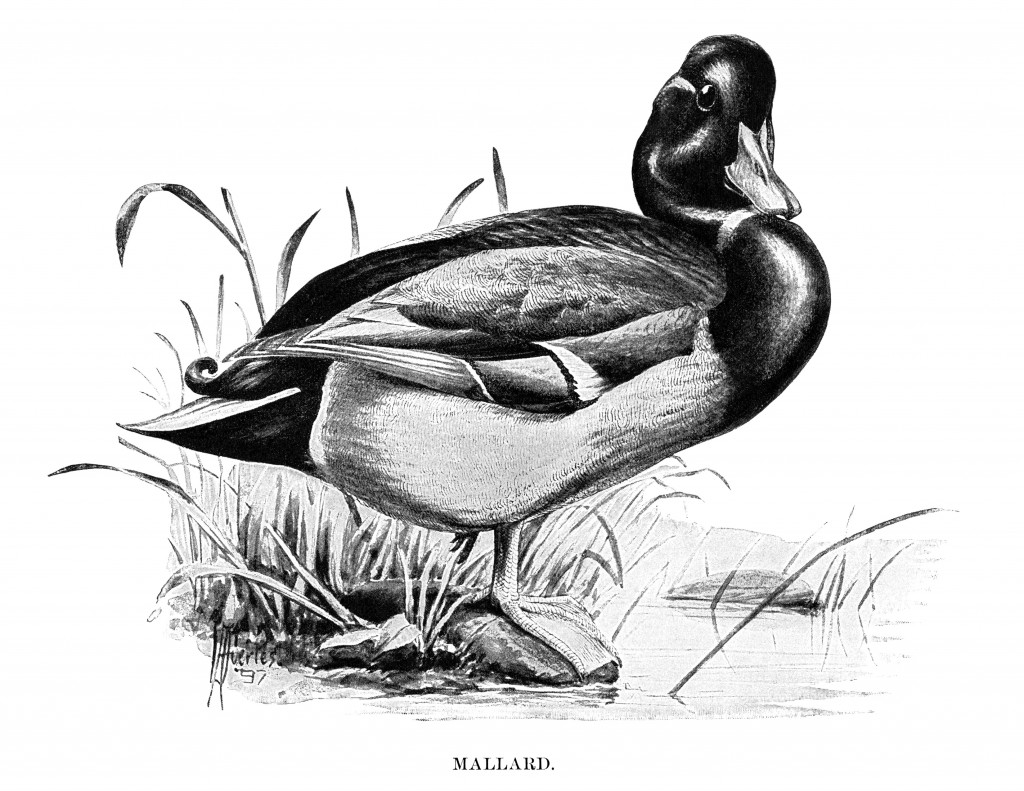
\includegraphics[width=\linewidth]{figures/duck}
  \caption{An illustration of a Mallard Duck. Picture from Mabel Osgood Wright, \textit{Birdcraft}, published 1897.}
  \label{fig:duck}
\end{figure}

\subsection{Tables}

Curabitur vitae nulla dapibus, ornare dolor in, efficitur enim \cite{Editor00}. Cras fermentum facilisis elit vitae egestas. Mauris porta, neque non rutrum efficitur, odio odio faucibus tortor, vitae imperdiet metus quam vitae eros. Proin porta dictum accumsan.

Duis cursus maximus facilisis. Integer euismod, purus et condimentum suscipit, augue turpis euismod libero, ac porttitor tellus neque eu enim. Nam vulputate est non tellus efficitur pharetra. Aenean molestie tristique venenatis. Nam congue pulvinar vehicula. Duis lacinia mollis purus, ac aliquet arcu dignissim ac \autoref{tab:freq}. 

\begin{table}[hb]% h asks to places the floating element [h]ere.
  \caption{Frequency of Special Characters}
  \label{tab:freq}
  \begin{tabular}{ccl}
    \toprule
    Non-English or Math & Frequency & Comments\\
    \midrule
    \O & 1 in 1000& For Swedish names\\
    $\pi$ & 1 in 5 & Common in math\\
    \$ & 4 in 5 & Used in business\\
    $\Psi^2_1$ & 1 in 40\,000 & Unexplained usage\\
  \bottomrule
\end{tabular}
\end{table}

Nulla sit amet enim tortor \cite{Editor00a}. Ut non felis lectus. Aenean quis
felis faucibus, efficitur magna vitae. Curabitur ut mauris vel augue tempor suscipit eget eget lacus. Sed pulvinar lobortis dictum.
Aliquam dapibus a velit.

%\clearpage

\bibliographystyle{ACM-Reference-Format}
\bibliography{sample}

\end{document}
\endinput
